%
% 98-127
% Lecture 02: A First Look at Unity
% 
% Template adapted from
% https://www.cs.cmu.edu/~15150/previous-semesters/2012-spring/resources/latex/template.tex
%

\documentclass[11pt]{article}

\usepackage{amsmath}
\usepackage{amssymb}
\usepackage{amsthm}
\usepackage{hyperref}
\usepackage{fancyhdr}
\usepackage{listings}
\usepackage{color}
\usepackage{graphicx}
\usepackage{setspace}
\usepackage{times}
\usepackage{wrapfig}
\usepackage{fontawesome}

\oddsidemargin0cm
\topmargin-2cm
\textwidth16.5cm
\textheight23.5cm

\newtheorem{lemma}{Lemma}

%% Begin Constants %% <-- (edit these!)

% Lecture Info
\newcommand{\lecturenum}{2}
\newcommand{\lecturename}{A First Look at Unity}

% Author of THIS document
\newcommand{\authorname}{Adrian Biagioli}

% Course Info
\newcommand{\coursenum}{98-127}
\newcommand{\coursename}{Game Creation for People Who Want to Make Games}
\newcommand{\coursesem}{S19}

% Instructors of course
\newcommand{\instructors}{Adrian Biagioli (\,\href{mailto:abiagiol@andrew.cmu.edu}{abiagiol@andrew.cmu.edu}\,) \\ Carter Williams (\,\href{mailto:ncwillia@andrew.cmu.edu}{ncwillia@andrew.cmu.edu}\,)}

% Math shortcuts
\newcommand{\work}{\mathcal{W}}
\newcommand{\expv}{\mathbf{E}}
\newcommand{\pr}{\mathbf{Pr}}
\newcommand{\ts}{\textsuperscript}
\newcommand{\bigo}{\mathit{O}}

%% End Constants %%

%% Begin syntax highlighting settings %%

\definecolor{dkgreen}{rgb}{0,0.6,0}
\definecolor{gray}{rgb}{0.5,0.5,0.5}
\definecolor{mauve}{rgb}{0.58,0,0.82}

\lstset{frame=tb,
    language=ML,
    aboveskip=3mm,
    belowskip=3mm,
    showstringspaces=false,
    columns=flexible,
    basicstyle={\small\ttfamily},
    numbers=left,
    stepnumber=1,
    numberstyle=\tiny\color{gray},
    keywordstyle=\color{blue},
    commentstyle=\color{dkgreen},
    stringstyle=\color{mauve},
    breaklines=true,
    breakatwhitespace=true,
    tabsize=3
  }

\lstnewenvironment{pseudocode}[1][]
{
    \lstset{
        mathescape=true,
        frame=tb,
        numbers=left, 
        basicstyle=\small, 
        numberstyle=\tiny\color{gray},
        keywordstyle=\color{black}\bfseries\em,
        commentstyle=\color{dkgreen},
        stringstyle=\color{mauve},
        keywords={,input, output, return, datatype, function, in, if, else, foreach, while, begin, end, }
        numbers=left,
        breaklines=true,
        breakatwhitespace=true,
        tabsize=3
    }
}
{}

% From https://tex.stackexchange.com/questions/95036/continue-line-numbers-in-listings-package
\def\ContinueLineNumber{\lstset{firstnumber=last}}
\def\StartLineAt#1{\lstset{firstnumber=#1}}
\let\numberLineAt\StartLineAt

%% End syntax highlighting settings %%

\setlength{\parindent}{2em}
\setlength{\parskip}{5pt plus 1pt}
\renewcommand{\baselinestretch}{1.15}

\pagestyle{fancyplain}
{
    \lhead{\fancyplain{}{Lecture \lecturenum}}
    \rhead{\fancyplain{}{\coursenum}}
    \chead{\fancyplain{}{\lecturename}}
}
\setlength{\headheight}{14pt}

\graphicspath{ {./images/} }

\begin{document}

\thispagestyle{plain}
{
    \vspace{1.5em}
    \begin{center}
    {
        \huge
        Lecture \lecturenum \\
        \vspace{0.5em}
        \lecturename
        \vspace{0.4em}
    } \\
    {
        \it
        \coursenum: \coursename\ \ (\coursesem)
    } \\
    \vspace{1.0em}
    Written by \authorname \\
    \vspace{0.7em}
    Instructors:\\ \instructors
    \end{center}
}

\section{Objectives}

By the end of this lesson you will be able to:
\begin{itemize}
    \item Understand what a Game Engine is, and why we use the Unity game engine
    \item Utilize common Unity editor functionality and navigate scenes
    \item Understand Unity's high level architecture: the Scene Graph and GameObjects
    \item Utilize the inspector to design levels, given art assets and scripts
\end{itemize}

\noindent These lecture notes were written for {\bf Unity 2018.3.0f1}.

\section{What is a Game Engine?}

\par Video Games are a very complicated technical challenge.  Think about all of the stuff that goes on in your average video game, like Call of Duty.  There is a complicated {\it Graphics Pipeline}, which is the code that communicates very quickly with the user's graphics processor to produce complicated effects (shadows, explosions, hair, muzzle flashes\dots the list goes on).  There is also usually a {\it Physics Engine} that attempts to simulate how objects would interact with each other (for example, it would figure out how a grenade bounced throughout the scene).  There's also some sort of {\it Audio Mixer} that handles audio effects (for example, a low-pass filter when you are hit with a flashbang).  Then there's the {\it Animation Engine}, which allows characters to move around the scene realistically.  Many games include {\it Artificial Intelligence}, {\it UI Systems}, and more.

\par That's a lot of things that {\it many} games have in common!  In fact, it seems like a waste of time to re-do all of these complicated systems for every game that we want to make.  This is why Game Engines exist.  A {\bf Game Engine} aims to simplify game development by doing all the hard stuff for us (i.e. everything I mentioned in the previous paragraph).  This allows game designers like ourselves to focus on the good stuff: how to make our game fun.  In addition to this, game engines also tend to simplify {\it how we code} our games.  Many ``game-engine-less'' games are simply written in C++, which can be hard for beginners.  In contrast, Unity is in C\#, which is much more approachable.


{\bf Unity} is the most popular Game Engine out there right now for indie game developers, and it is the one that we will use in this course.  Right now, Unity's biggest competitor is the {\bf Unreal Engine 4} (UE4), which is developed by Epic Games (creators of {\it Gears of War} and {\it Fortnite}).  UE4 rivals Unity in many respects and outshines it in some (many will argue that UE4 has better builtin graphics than Unity), but we will not use it in this class because it is generally harder to use for beginners and requires knowledge of C++.  Another important difference is how you need to pay royalties if you decide to sell your game: Unity allows you to sell your game without paying any royalties, {\it until} your game makes \$100k per year.  After that point, you need to upgrade to Unity \href{https://store.unity.com}{``Plus'' or ``Pro''}, which has a monthly fee.  Unreal requires a 5\% royalty of all revenue of your game past \$3000, but has no Plus or Pro tier.

\section{Getting Started with Unity}

If you haven't already, download Unity:
\begin{itemize}
\item You can download Unity at \href{https://store.unity.com}{https://store.unity.com}.  Click on ``Try Personal'' and download the installer to get the latest version.  Make sure to enable Windows and Mac build support in the installer options.
\item If you're a programmer running Windows or Mac, I would recommend downloading Microsoft Visual Studio.  Visual Studio and Visual Studio for Mac both have great integration with Unity and are better than the default MonoDevelop: \href{https://www.visualstudio.com}{https://www.visualstudio.com}.
\end{itemize}

\begin{wrapfigure}{r}[50pt]{0.5\textwidth}
    \centering
    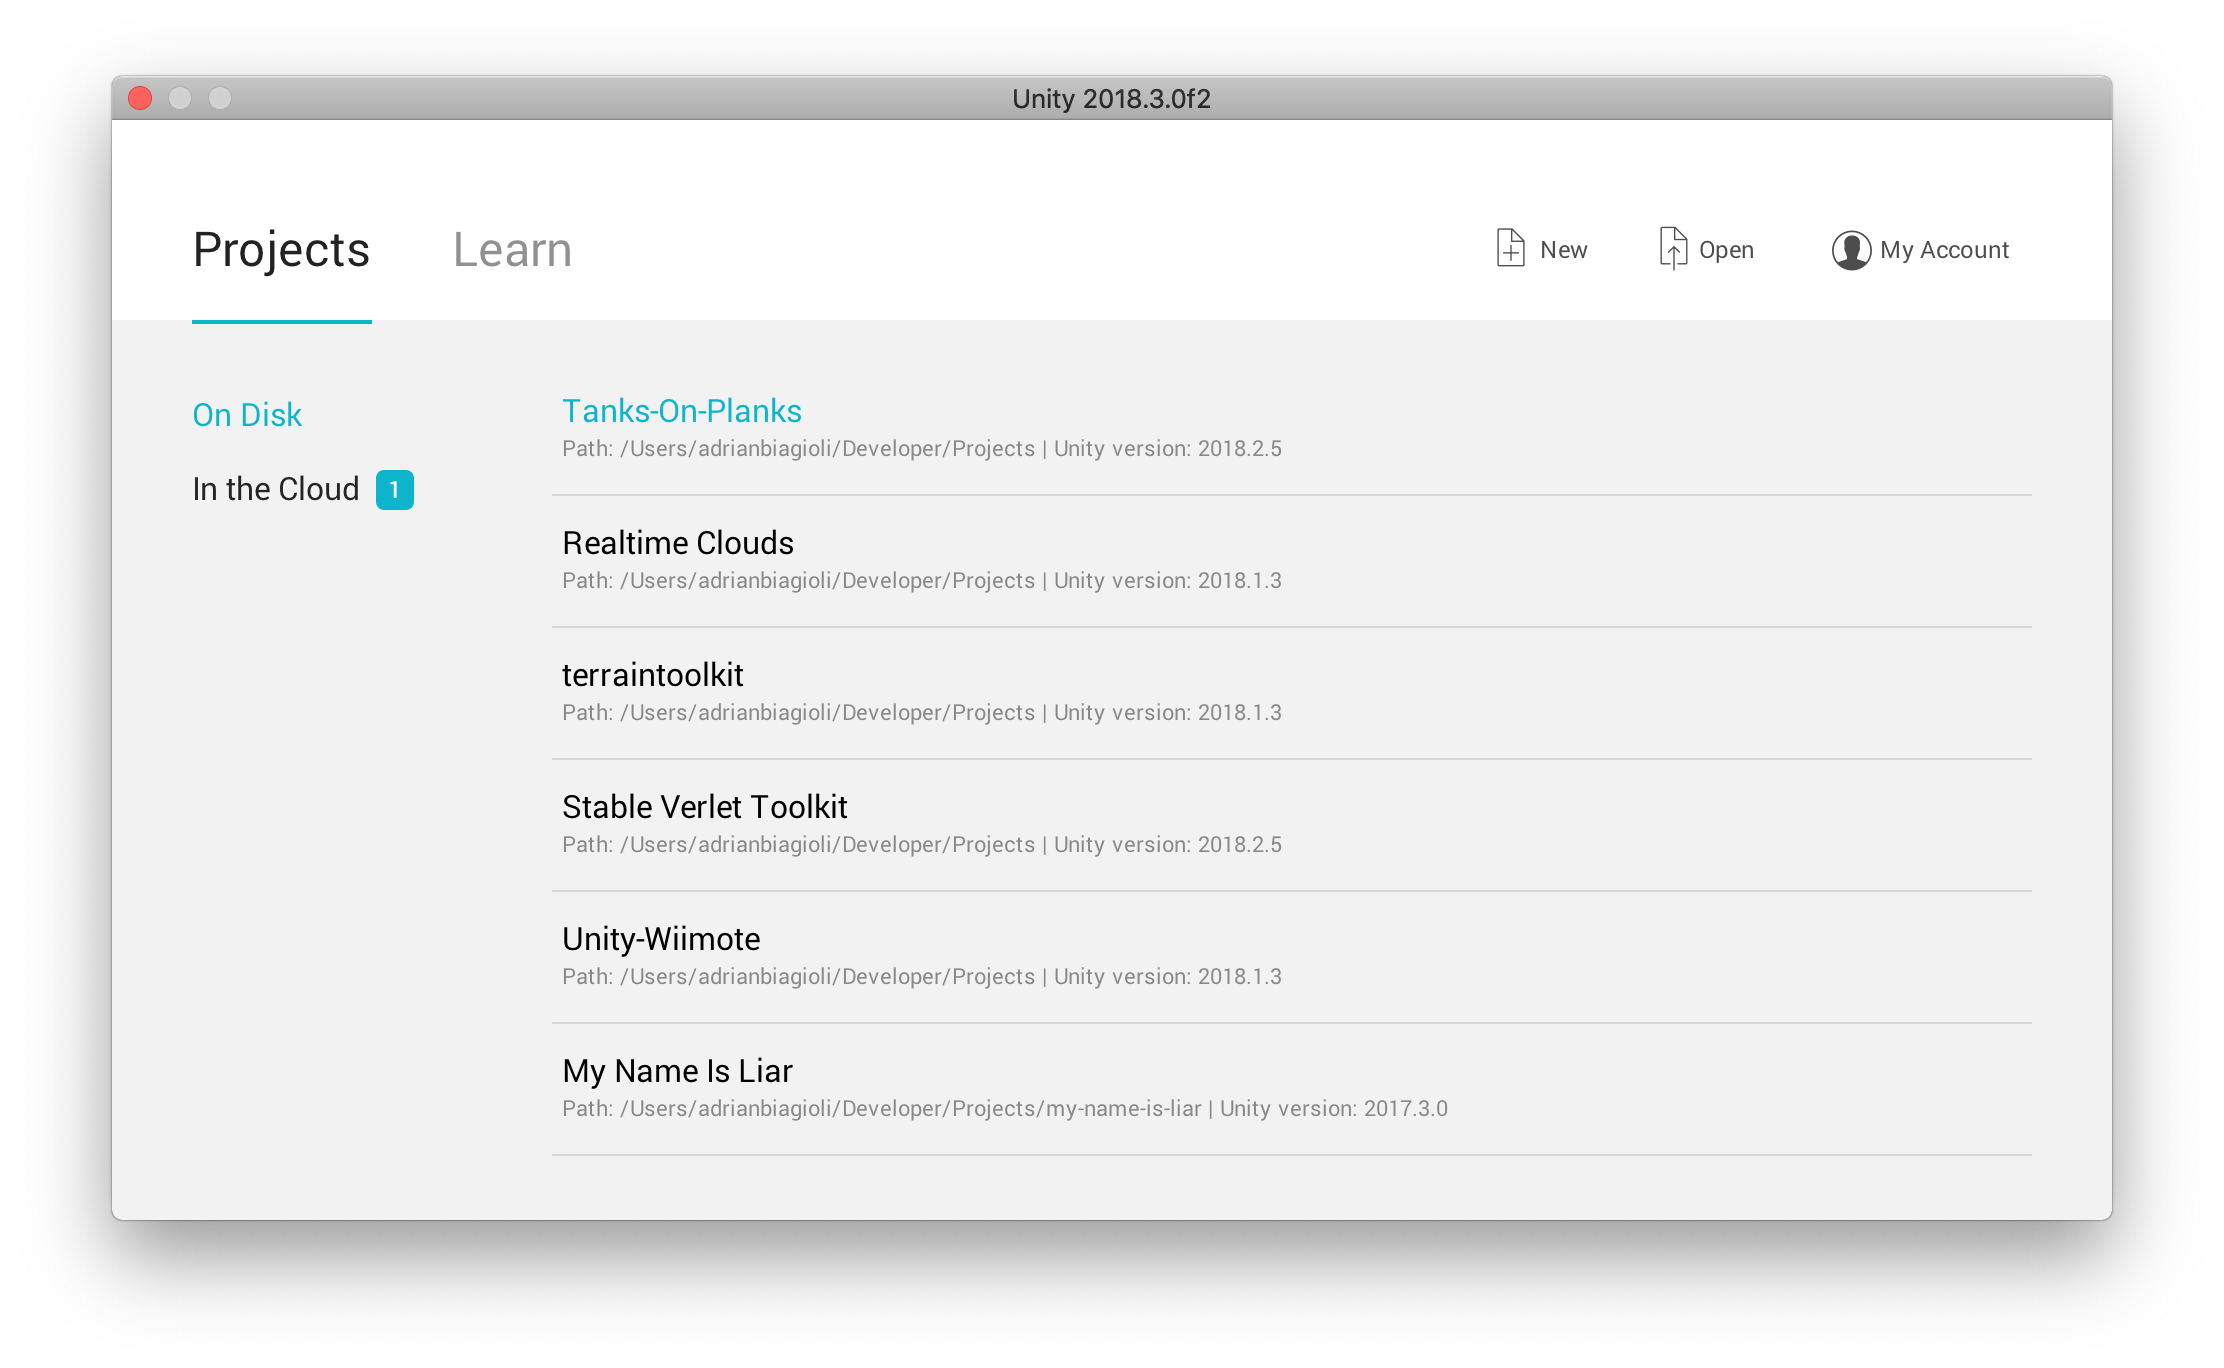
\includegraphics[width=0.5\textwidth]{proj-select}
    Unity Project Select Window
\end{wrapfigure}


When you open Unity, you will first see the {\bf project selection screen}.  You may need to create a Unity account—do so if prompted.  Click ``new project'' on the top right of the window.

Enter a name for your new project (``Lecture 2 Project'') and specify a location for the project folder.  Make sure ``3D'' is checked and ``Enable Unity Analytics'' is unchecked.  Then click {\it create project}.  \textbf{Unity projects are saved in folders on your machine}, so if you browse to the project location you gave then you will find the Unity project files.

The Unity editor should now appear.  The editor is divided into \textbf{panels}, each providing a different way to interact with your Unity project.  If your editor doesn’t look like the one on the next page, click \textit{Layout $\rightarrow$ Default} on the top right of the editor.  Notice that panels can be reorganized and redocked to other panels by clicking and dragging on the tab at the top of each pane.  You can also resize panels and drag them out to their own window.

\pagebreak
\section{Basic Unity Editor Panels}

{
\centering \noindent
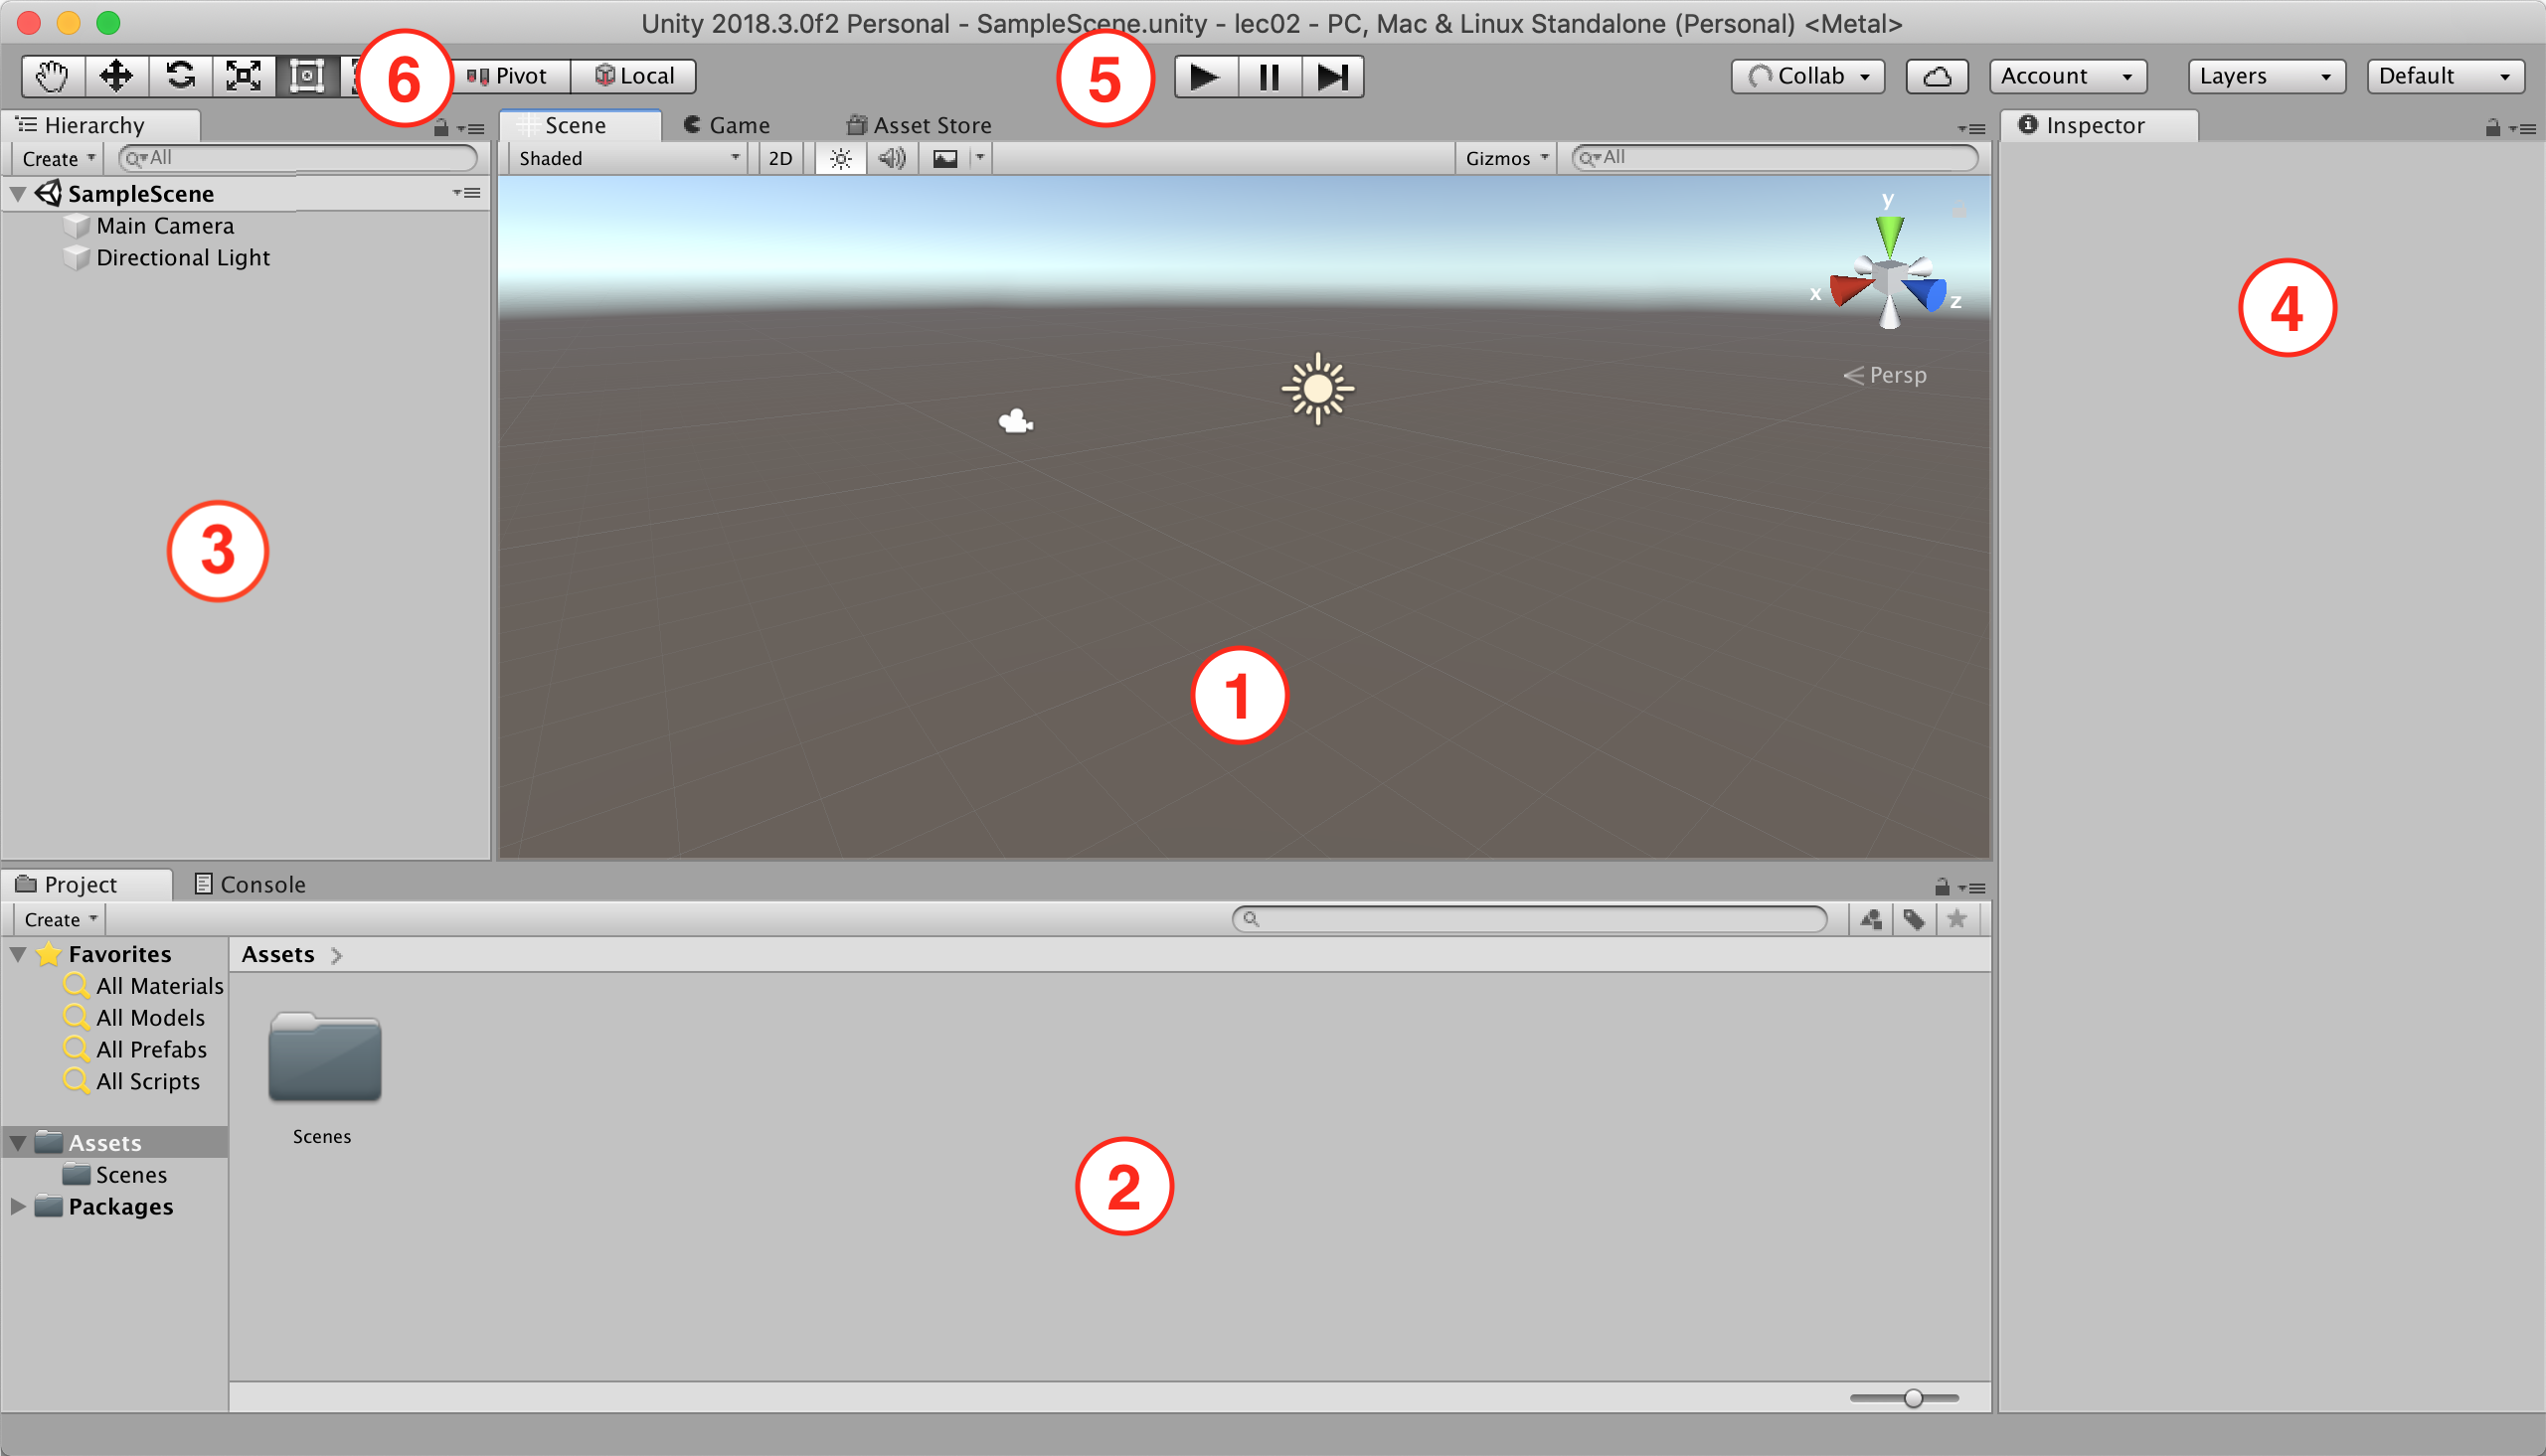
\includegraphics[width=1.0\textwidth]{basic-editor-panes}
}

This is the default configuration of the Unity editor, opening a freshly-made project.  Each panel that you see in the above screenshot is labeled as follows:

\begin{enumerate}
    \item The \textbf{Scene View} allows you to look into the game world from a perspective other than the in-game camera.  You can navigate the scene view as follows:
    \begin{itemize}
        \item \textbf{Right Click + Drag}: Look around
        \item \textbf{Right Click + WSADQE}: Move camera (FPS controls).  Hold shift to move faster.
        \item \textbf{Left Click}: Select and manipulate objects (see item 6 below)
    \end{itemize}
    \item The \textbf{Project Window} is a view into the assets of your game.  \textbf{Assets} are normal files that your game will use like scripts, 3D Models, textures (images), audio, animation data, scene files, and more.  The project window behaves much like the Finder on macOS or Explorer on Windows.
    \begin{itemize}
        \item In fact, these files are located in the \lstinline!/Assets! subfolder of your Unity project!  Try right clicking on a file in the project window and select ``Reveal\dots''
    \end{itemize}
    \item The \textbf{Hierarchy View} lists all of the \textbf{GameObjects} that are currently in the scene.
    \begin{itemize}
        \item In Unity terminology, a \textbf{GameObject} is any ``thing'' in your game.  \textit{Everything is a GameObject}: the player, a fence, an enemy, a weapon, a button, an NPC, a scoreboard, \dots.  Right now there are two GameObjects in the scene, a Main Camera and a Directional Light for the Sun.
        \item You can select a GameObject by clicking on it: either in the scene view or the hierarchy view.
        \item If you double click on a GameObject in the hierarchy view you can focus on it in the scene view.
    \end{itemize}
    \item The \textbf{Inspector} allows you to inspect and modify the properties of whichever GameObject or Asset is selected.  For example, you can change the position of a GameObject or the name of a file.  More information on how to use the Inspector will follow.
    \item The \textbf{Play Button} (\faPlay) will shift focus from the Scene View to the \textbf{Game View}, allowing you to play your game in real time!  When you are in ``Play Mode'', you can switch back to the Scene/Hierarchy/Inspector Panels and continue to modify the scene.  However, as soon as you stop playing (by clicking the play button again) \underline{your changes will revert to before you started playing}, so be careful!  While playing, you can also click the \textbf{Pause Button} (\faPause) to pause execution of the game (you can still make changes in the Scene View / Inspector while paused).  While paused, you can click the \textbf{Advance Frame Button} (\faFastForward) to advance by one frame.
    \item The \textbf{Scene View Tools} change the currently-active manipulator in the scene view.  These manipulators allow you to move, rotate, and scale GameObjects--more on this later.
\end{enumerate}

\end{document}